\section{Transformada de Fourier}

\begin{frame}[fragile]{Série de Fourier}

    \begin{itemize}
        \item Uma série de Fourier consiste na expansão de uma função períodica $f(x)$ em termos
            de senos e cosenos

        \item Isto possível porque as funções $\sin(mx)$ e $\sin(ny)$ são ortogonais para 
            $m\neq n$ no intervalo $[-\pi, \pi]$:

        \begin{align*}
            \int_{-\pi}^\pi \sin(mx)\sin(nx) dx &= 
            \int_{-\pi}^\pi \sin(mx)\cos(nx) dx \\
            &= \int_{-\pi}^\pi \cos(mx)\cos(nx) dx = 0
        \end{align*}

        \item Para $m = n$, segue que
        \[
            \int_{-\pi}^\pi \sin^2(mx) dx = 
            \int_{-\pi}^\pi \cos^2(mx) dx = \pi
        \]

    \end{itemize}

\end{frame}

\begin{frame}[fragile]{Série de Fourier}

    \begin{itemize}
        \item Deste modo,
        \[
            f(x) = \frac{1}{2}a_0 + \sum_{n=1}^\infty a_n\cos(n x) + \sum_{n=1}^\infty b_n\sin(nx),
        \]
        onde
        \begin{align*}
            a_0 &= \frac{1}{\pi}\int_{-\pi}^{\pi} f(x)dx \\    
            a_n &= \frac{1}{\pi}\int_{-\pi}^{\pi} f(x)\cos(nx)dx \\    
            b_n &= \frac{1}{\pi}\int_{-\pi}^{\pi} f(x)\sin(nx)dx    
        \end{align*}
    
    \end{itemize}

\end{frame}

\begin{frame}[fragile]{Exemplo: Onda Quadrada}

    Considere a onda quadrada $x(t) = a\,\mathrm{sign}(\sin(t))$:

    \begin{figure}
        \centering

        \begin{tikzpicture}
            \draw[very thick] (-1, 0) -- (0, 0) -- (0, 2) -- (pi, 2) -- (pi, 0) -- ({2*pi}, 0)
                -- (2*pi, 2) -- (3*pi, 2) -- (3*pi, 0) -- (10, 0);

            \node[anchor=east] at (0, 2) { $a$ };
            \node[anchor=north] at (pi, 0) { $\pi$ };
            \node[anchor=north] at (2*pi, 0) { $2\pi$ };
            \node[anchor=north] at (3*pi, 0) { $3\pi$ };

%            \draw[blue!60!black,domain=-1:10,samples=201] plot (\x, {1 + (4/pi)*sin(\x*180/pi)
%               + (4/(3*pi))*sin(\x*3*180/pi)
%                + (4/(5*pi))*sin(\x*5*180/pi)
%                + (4/(7*pi))*sin(\x*7*180/pi)
%});

            \draw[->] (0,-1) -- (0, 3.2) node[anchor=east] { $x$ };
            \draw[->] (-1,0) -- (10.2, 0) node[anchor=north] { $t$ };
        \end{tikzpicture}
    \end{figure}

\end{frame}

\begin{frame}[fragile]{Exemplo: Onda Quadrada}

    \begin{itemize}
        \item O coeficiente $a_0$ é dado por
        \[
            a_0 = \frac{1}{\pi}\int_{-\pi}^{\pi} f(t)dt = \frac{1}{\pi}\int_{0}^{\pi} a\, dt = a
        \]

        \item Os coeficientes $a_n$, para $n\geq 1$, são todos iguais a zero, pois
        \[
            a_n = \frac{1}{\pi}\int_{-\pi}^{\pi} f(t)\cos(nt) dt 
                = \frac{a}{\pi}\left[\left.\frac{\sin(nt)}{n}\right\rvert_0^\pi\right] = 0
        \]

        \item Os coeficientes $b_n$ são iguais a zero, para $n$ par, e
        \[
            b_n = \frac{1}{\pi}\int_{-\pi}^{\pi} f(t)\sin(nt) dt 
                = -\frac{a}{\pi}\left[\left.\frac{\cos(nt)}{n}\right\rvert_0^\pi\right] = \frac{2a}{m\pi},
        \]
        se $n$ é ímpar
    \end{itemize}

\end{frame}

\begin{frame}[fragile]{Exemplo: Aproximação da onda quadrada com $n = 0$}

    Considere a onda quadrada $x(t) = a\,\mathrm{sign}(\sin(t))$:

    \begin{figure}
        \centering

        \begin{tikzpicture}
            \draw[very thick] (-1, 0) -- (0, 0) -- (0, 2) -- (pi, 2) -- (pi, 0) -- ({2*pi}, 0)
                -- (2*pi, 2) -- (3*pi, 2) -- (3*pi, 0) -- (10, 0);

            \node[anchor=east] at (0, 2) { $a$ };
            \node[anchor=north] at (pi, 0) { $\pi$ };
            \node[anchor=north] at (2*pi, 0) { $2\pi$ };
            \node[anchor=north] at (3*pi, 0) { $3\pi$ };

            \draw[blue!60!black,domain=-1:10,samples=201] plot (\x, {1 
% + (4/pi)*sin(\x*180/pi)
%               + (4/(3*pi))*sin(\x*3*180/pi)
%                + (4/(5*pi))*sin(\x*5*180/pi)
%                + (4/(7*pi))*sin(\x*7*180/pi)
});

            \draw[->] (0,-1) -- (0, 3.2) node[anchor=east] { $x$ };
            \draw[->] (-1,0) -- (10.2, 0) node[anchor=north] { $t$ };
        \end{tikzpicture}
    \end{figure}

\end{frame}

\begin{frame}[fragile]{Exemplo: Aproximação da onda quadrada com $n = 1$}

    Considere a onda quadrada $x(t) = a\,\mathrm{sign}(\sin(t))$:

    \begin{figure}
        \centering

        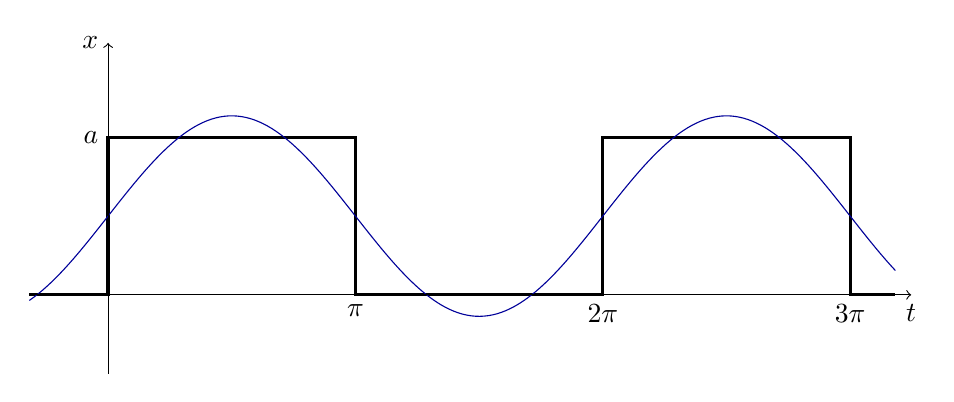
\begin{tikzpicture}
            \draw[very thick] (-1, 0) -- (0, 0) -- (0, 2) -- (pi, 2) -- (pi, 0) -- ({2*pi}, 0)
                -- (2*pi, 2) -- (3*pi, 2) -- (3*pi, 0) -- (10, 0);

            \node[anchor=east] at (0, 2) { $a$ };
            \node[anchor=north] at (pi, 0) { $\pi$ };
            \node[anchor=north] at (2*pi, 0) { $2\pi$ };
            \node[anchor=north] at (3*pi, 0) { $3\pi$ };

            \draw[blue!60!black,domain=-1:10,samples=201] plot (\x, {1 
                + (4/pi)*sin(\x*180/pi)
%               + (4/(3*pi))*sin(\x*3*180/pi)
%               + (4/(5*pi))*sin(\x*5*180/pi)
%               + (4/(7*pi))*sin(\x*7*180/pi)
});

            \draw[->] (0,-1) -- (0, 3.2) node[anchor=east] { $x$ };
            \draw[->] (-1,0) -- (10.2, 0) node[anchor=north] { $t$ };
        \end{tikzpicture}
    \end{figure}

\end{frame}

\begin{frame}[fragile]{Exemplo: Aproximação da onda quadrada com $n = 3$}

    Considere a onda quadrada $x(t) = a\,\mathrm{sign}(\sin(t))$:

    \begin{figure}
        \centering

        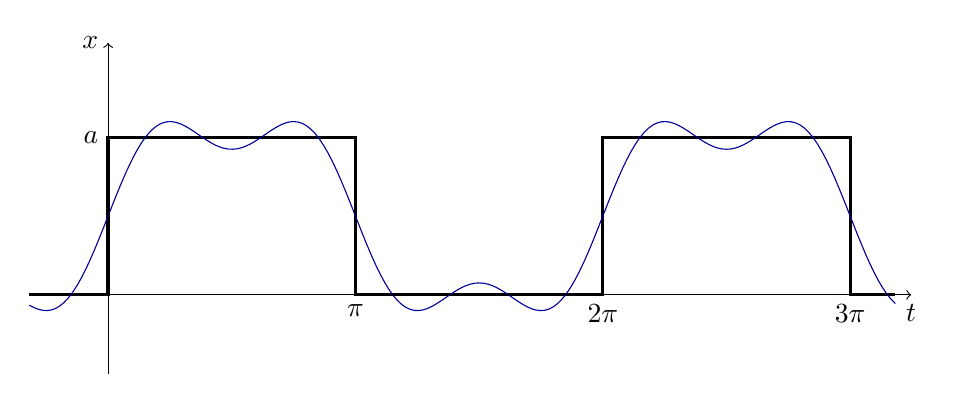
\begin{tikzpicture}
            \draw[very thick] (-1, 0) -- (0, 0) -- (0, 2) -- (pi, 2) -- (pi, 0) -- ({2*pi}, 0)
                -- (2*pi, 2) -- (3*pi, 2) -- (3*pi, 0) -- (10, 0);

            \node[anchor=east] at (0, 2) { $a$ };
            \node[anchor=north] at (pi, 0) { $\pi$ };
            \node[anchor=north] at (2*pi, 0) { $2\pi$ };
            \node[anchor=north] at (3*pi, 0) { $3\pi$ };

            \draw[blue!60!black,domain=-1:10,samples=201] plot (\x, {1 
                + (4/pi)*sin(\x*180/pi)
               + (4/(3*pi))*sin(\x*3*180/pi)
%               + (4/(5*pi))*sin(\x*5*180/pi)
%               + (4/(7*pi))*sin(\x*7*180/pi)
});

            \draw[->] (0,-1) -- (0, 3.2) node[anchor=east] { $x$ };
            \draw[->] (-1,0) -- (10.2, 0) node[anchor=north] { $t$ };
        \end{tikzpicture}
    \end{figure}

\end{frame}

\begin{frame}[fragile]{Exemplo: Aproximação da onda quadrada com $n = 5$}

    Considere a onda quadrada $x(t) = a\,\mathrm{sign}(\sin(t))$:

    \begin{figure}
        \centering

        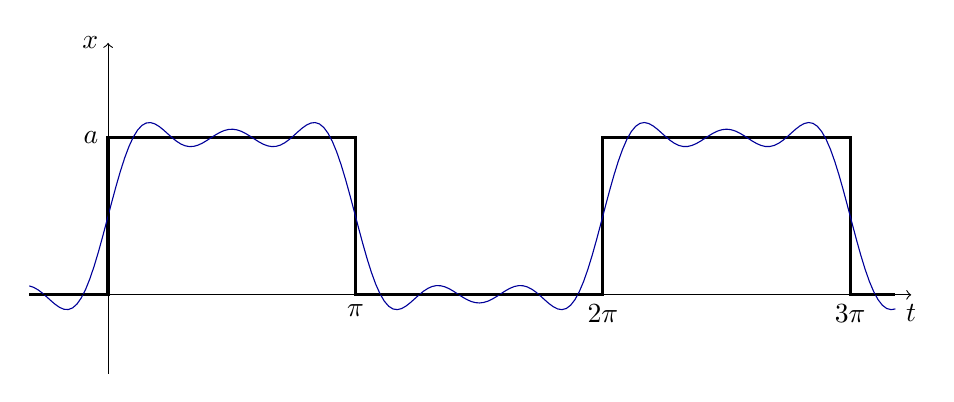
\begin{tikzpicture}
            \draw[very thick] (-1, 0) -- (0, 0) -- (0, 2) -- (pi, 2) -- (pi, 0) -- ({2*pi}, 0)
                -- (2*pi, 2) -- (3*pi, 2) -- (3*pi, 0) -- (10, 0);

            \node[anchor=east] at (0, 2) { $a$ };
            \node[anchor=north] at (pi, 0) { $\pi$ };
            \node[anchor=north] at (2*pi, 0) { $2\pi$ };
            \node[anchor=north] at (3*pi, 0) { $3\pi$ };

            \draw[blue!60!black,domain=-1:10,samples=201] plot (\x, {1 
                + (4/pi)*sin(\x*180/pi)
               + (4/(3*pi))*sin(\x*3*180/pi)
               + (4/(5*pi))*sin(\x*5*180/pi)
%               + (4/(7*pi))*sin(\x*7*180/pi)
});

            \draw[->] (0,-1) -- (0, 3.2) node[anchor=east] { $x$ };
            \draw[->] (-1,0) -- (10.2, 0) node[anchor=north] { $t$ };
        \end{tikzpicture}
    \end{figure}

\end{frame}

\begin{frame}[fragile]{Exemplo: Aproximação da onda quadrada com $n = 7$}

    Considere a onda quadrada $x(t) = a\,\mathrm{sign}(\sin(t))$:

    \begin{figure}
        \centering

        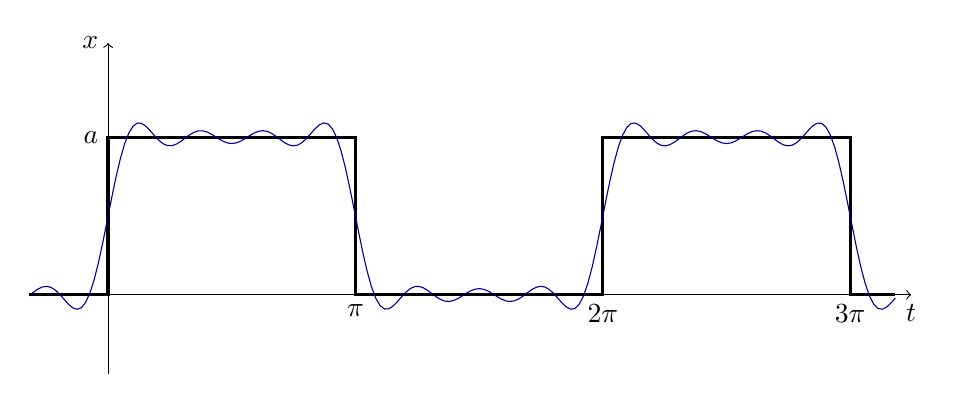
\begin{tikzpicture}
            \draw[very thick] (-1, 0) -- (0, 0) -- (0, 2) -- (pi, 2) -- (pi, 0) -- ({2*pi}, 0)
                -- (2*pi, 2) -- (3*pi, 2) -- (3*pi, 0) -- (10, 0);

            \node[anchor=east] at (0, 2) { $a$ };
            \node[anchor=north] at (pi, 0) { $\pi$ };
            \node[anchor=north] at (2*pi, 0) { $2\pi$ };
            \node[anchor=north] at (3*pi, 0) { $3\pi$ };

            \draw[blue!60!black,domain=-1:10,samples=201] plot (\x, {1 
                + (4/pi)*sin(\x*180/pi)
               + (4/(3*pi))*sin(\x*3*180/pi)
               + (4/(5*pi))*sin(\x*5*180/pi)
               + (4/(7*pi))*sin(\x*7*180/pi)
});

            \draw[->] (0,-1) -- (0, 3.2) node[anchor=east] { $x$ };
            \draw[->] (-1,0) -- (10.2, 0) node[anchor=north] { $t$ };
        \end{tikzpicture}
    \end{figure}

\end{frame}

